\section{Projektorganisation}
\label{sec:einleitung.Projektorganisation}

\subsection{Beteiligte Personen}
\label{sec:einleitung.Projektorganisation.BetroffenePersonen}

\textbf{Studierende:}\\
 Lukas Kuster \textit{kustl1@bfh.ch} \\
 Stefan K�ser \textit{kases1@bfh.ch}
 
\textbf{Betreuung:}\\
Dr. J�rgen Eckerle \textit{juergen.eckerle@bfh.ch}

\textbf{Experte:}\\
Dr. Federico Fl�ckiger	\textit{federico.flueckiger@bluewin.ch}


\subsection{Projektmeetings}
\label{sec:einleitung.Projektorganisation.Projektmeetings}

\begin{itemize}
\item Es fand jeweils ein Treffen mit dem Betreuer alle 1-2 Wochen statt.
\item Ein Treffen mit dem Experten fand am Anfang der Arbeit statt. Ein zweites Meeting wurde von beiden Seiten nicht f�r notwendig erachtet.
\end{itemize}

\subsection{Arbeitsweise}
\label{sec:einleitung.Projektorganisation.Arbeitsweise}

F�r die gemeinsame Arbeit am Projekt hatten wir uns jeweils den Freitag reserviert. An diesen Tagen arbeiteten wir meist mit Pair-Programming und erzielten dabei gute Fortschritte. Die verbleibenden Aufgaben teilten wir uns auf und arbeiteten einzeln daran. Dabei war die Versionskontrolle mit Git ein sehr hilfreiches Tool, um die Arbeiten zu koordinieren.

Wir arbeiteten mit einem zentralen, �ffentlichen Repository auf GitHub (\url{https://github.com/koschder/ants/}). Nebst dem Vorteil einer vereinfachten Zusammenarbeit bietet GitHub auch einige graphische Auswertungen der Aktivit�t in einem Projekt, die Aufschluss �ber den Verlauf unserer Arbeit geben.

\begin{figure}[H]
\centering
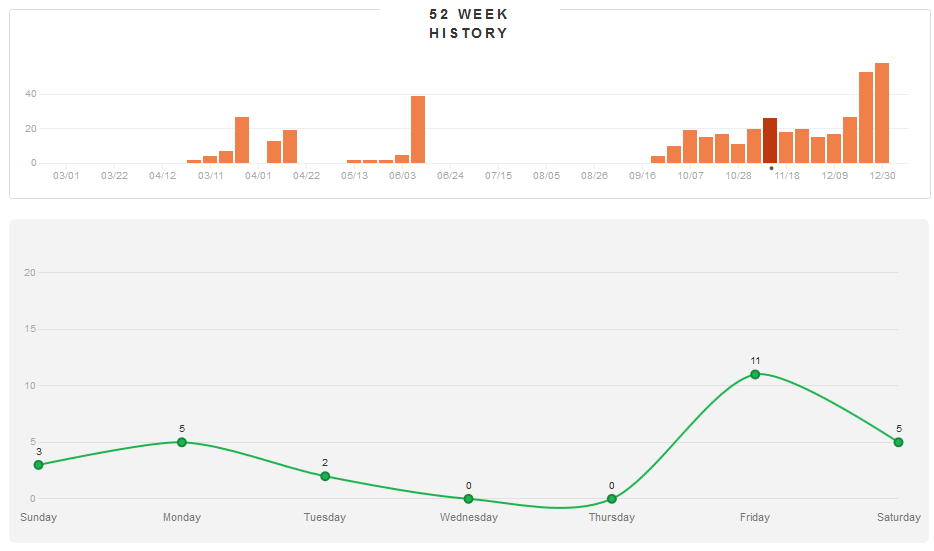
\includegraphics[width=0.99\textwidth]{91_bilder/github/commits}
\caption{Commit History}
\label{fig:commits}
\end{figure}

Die obere H�lfte der Abbildung \ref{fig:commits} zeigt den Aktivit�tsverlauf des Projekts r�ckblickend auf das letzte Jahr. Links, w�hrend den Monaten M�rz, April, Mai und Juni ist der Verlauf des Projekts 2 zu sehen, nach der Sommerpause der Verlauf der Bachelorarbeit. Die Aktivit�tssteigerung gegen Ende des Projekts ist vor allem auf Dokumentations- und Aufr�umarbeiten zur�ckzuf�hren.

Die untere H�lfte zeigt die Anzahl Commits �ber eine Woche verteilt. Man sieht sch�n, dass der Freitag mit Abstand der produktivste Tag war, mit reduzierter Aktivit�t �ber den Rest der Woche verstreut.

\begin{figure}[H]
\centering
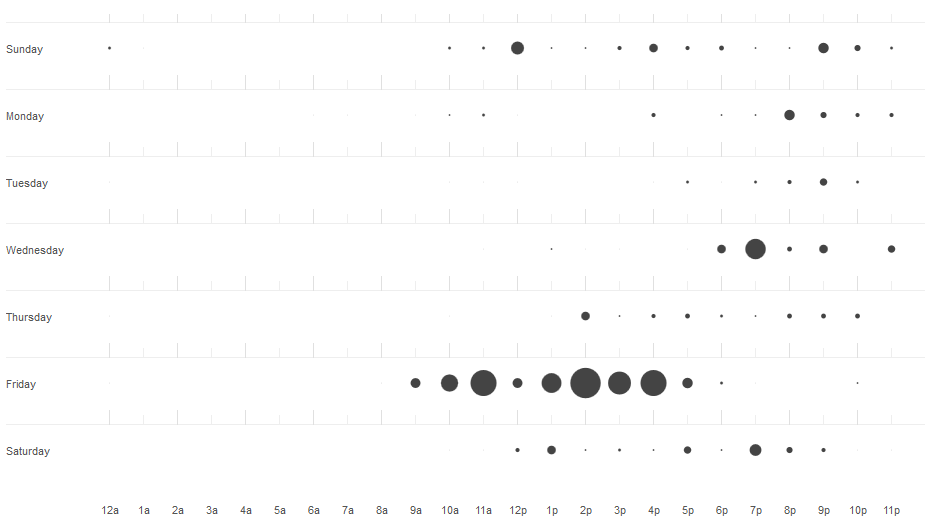
\includegraphics[width=0.99\textwidth]{91_bilder/github/punchcard}
\caption{Aktivit�ten}
\label{fig:punchcard}
\end{figure}

Abbildung \ref{fig:punchcard} zeigt f�r den gesamten Projektverlauf die Zeiten mit der gr�ssten Aktivit�t. Auch hier kann man deutlich erkennen, dass der gr�sste Teil der Arbeit an den Freitagen erstellt wurde.

